\documentclass{article}
\usepackage{amsmath}
\usepackage[UTF8]{ctex}
\usepackage{tikz,mathpazo}
\usepackage{extarrows}
\usepackage{wrapfig}
\usepackage{graphicx}

\usetikzlibrary{graphs} % LATEX and plain TEX
\usetikzlibrary[graphs] % ConTEXt
\usetikzlibrary{quotes} % LATEX and plain TEX
\usetikzlibrary[quotes] % ConTEXt

\newtheorem{proof}{证明}
\newtheorem{theorem}{定理}
\newtheorem{definition}{定义}

\begin{document}
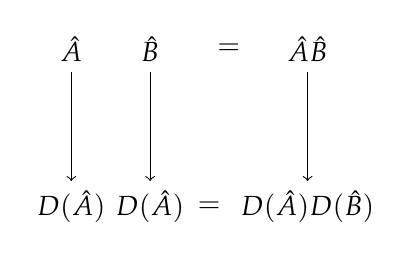
\begin{tikzpicture}
  \node (a) at (0,0) {$\hat{A}$};
  \node (b) at (1,0) {$\hat{B}$};
  \node (=) at (2,0) {$=$};
  \node (ab) at (3,0) {$\hat{A}\hat{B}$};
  \node (da) at (0,-2) {$D(\hat{A})$};
  \node (db) at (1,-2) {$D(\hat{A})$};
  \node (=) at (1.75,-2) {$=$};
  \node (dab) at (3,-2) {$D(\hat{A})D(\hat{B})$};
  \graph{(a) -> (da)};
  \graph{(b) -> (db)};
  \graph{(ab) -> (dab)};
\end{tikzpicture}
\begin{equation*}
  (ye^{-\frac{x^2}{2}})'=e^{-\frac{x^2}{2}}(y'-xy)
\end{equation*}
\begin{equation*}
  y'-xy=\frac{1}{2\sqrt{x}}e^{\frac{x^2}{2}}
\end{equation*}
两边乘以$e^{-\frac{x^2}{2}}$
\begin{equation*}
  e^{-\frac{x^2}{2}}(y'-xy)=(ye^{-\frac{x^2}{2}})'=\frac{1}{2\sqrt{x}}
\end{equation*}
积分因子法
\begin{equation*}
  e^{\int a(x)\mathrm{d}x}(y'+a(x)y)=(ye^{\int a(x)\mathrm{d}x})'
\end{equation*}
\end{document} 